\documentclass{article}
\usepackage{amsmath}
\usepackage{amsfonts}
\usepackage{cite}
\usepackage{graphicx}
\graphicspath{{Figs/}{README/Figs/}}
\usepackage{algorithmic}
\usepackage{algorithm}
\usepackage{float}
\usepackage[margin=0.75in]{geometry}
\usepackage{arydshln}
\usepackage{wrapfig}

\newcommand{\D}{\mathrm{d}}
\title{Aeromechanical Model for Robobee Simulator}
\author{}
\date{}

\begin{document}

\maketitle
Much of what is found here can be found in Whitney and Wood's 2010 paper, "Aeromechanics of passive rotation in flapping flight". 

The overall simulation framework looks like 
\begin{itemize}
    \item Grab current wing/body state 
    \item Hinge moment balance 
    \item Aerodynamic force and moment calculation. 
    \item Applied Drake forces/torques 
    \item Integration 
\end{itemize}

\section{Methods} 
\subsection{Current Kinematic State}
Note that \(\phi\) is the stroke angle (the angle as the wing sweeps back and forth), \(\psi\) is the passive wing pitch angle, and \(\theta\) is the deviation angle (the angle as the wing moves up and down). The total wing angular velocity can be expressed as a vector sum, where 
\begin{equation}
    \label{eq:vector_sum}
    \boldsymbol{\omega} = -\dot{\phi} \mathbf{e}_X + \dot{\theta} \mathbf{e}_z + \dot{\psi} \mathbf{e}_x.
\end{equation}
But since there is no DOF in the \(\theta\) direction, we can set them to 0. 
Then, the equation simply means it is a sum of the sweep angular velocity and the pitch angle velocity. 
We then want to break apart \(\omega\) into \(\omega_h\) and \(\omega_x\) (angular velocity around the wing's own pitch axis). Then, we can define 
\begin{equation}
   \boldsymbol{\omega}_h = \boldsymbol{\omega} - {\omega}_x \mathbf{e}_x. 
\end{equation}
(which is literally just saying removing the \(\mathbf{e}_x\) component from rotation). Then, for the no stroke-plane-deviation case, 
\begin{equation}
    \boldsymbol{\omega}_h = -\dot{\phi}.
\end{equation}
And after a change of basis (see Appendix \ref{sec:change_of_basis_derivation}), we can express the angular velocity in the wing-fixed frame as
\begin{align}
    \boldsymbol{\omega}_x &= \dot{\psi} - \dot{\phi}\sin\theta \\ 
    &= \dot{\psi},
\end{align}
again because \(\theta = 0\) in our simplified planar case. 

\subsubsection{Blade-element kinematics and force application}

The Drake/CAD/URDF wing body frame \(B\) is not necessarily aligned with the
aerodynamic span/chord axes used by the blade-element model. Let
\(\theta_s=\texttt{span\_axis\_angle\_rad}\) be the fixed angle between the
body-frame \(x\)-axis and the aerodynamic span axis. Expressed in the wing body
frame,
\begin{align}
    \hat{\mathbf{s}}_B
        &= \cos\theta_s\,\hat{\mathbf{x}}_B
        + \sin\theta_s\,\hat{\mathbf{y}}_B, \\
    \hat{\mathbf{c}}_B
        &= \sigma_c
        \left(
            -\sin\theta_s\,\hat{\mathbf{x}}_B
            + \cos\theta_s\,\hat{\mathbf{y}}_B
        \right), \\
    \hat{\mathbf{n}}_B
        &= \hat{\mathbf{s}}_B \times \hat{\mathbf{c}}_B,
\end{align}
where
\[
    \sigma_c = \operatorname{sign}(\texttt{chord\_axis\_sign}).
\]
The body-to-aerodynamic-component projection matrix is
\begin{equation}
    X_{AB}
    =
    \begin{bmatrix}
        \hat{\mathbf{s}}_B^T\\
        \hat{\mathbf{c}}_B^T\\
        \hat{\mathbf{n}}_B^T
    \end{bmatrix}.
\end{equation}
Thus, for any vector \(\mathbf{v}^B\) expressed in the wing body frame,
\begin{equation}
    \mathbf{v}^A
    =
    X_{AB}\mathbf{v}^B
    =
    \begin{bmatrix}
        \mathbf{v}^B\cdot\hat{\mathbf{s}}_B\\
        \mathbf{v}^B\cdot\hat{\mathbf{c}}_B\\
        \mathbf{v}^B\cdot\hat{\mathbf{n}}_B
    \end{bmatrix}.
\end{equation}
The matrix \(X_{AB}\) is fixed for a given wing geometry. The physical pose of the
wing is still given by \(R_{WB}\). Therefore aerodynamic basis vectors are mapped
to world coordinates by
\begin{equation}
    \hat{\mathbf{s}}_W = R_{WB}\hat{\mathbf{s}}_B,
    \qquad
    \hat{\mathbf{c}}_W = R_{WB}\hat{\mathbf{c}}_B,
    \qquad
    \hat{\mathbf{n}}_W = R_{WB}\hat{\mathbf{n}}_B.
\end{equation}
Equivalently, if
\[
    R_{BA}
    =
    \begin{bmatrix}
        \hat{\mathbf{s}}_B &
        \hat{\mathbf{c}}_B &
        \hat{\mathbf{n}}_B
    \end{bmatrix},
\]
then
\begin{equation}
    X_{AB}=R_{BA}^T,
    \qquad
    R_{WA}=R_{WB}X_{AB}^T.
\end{equation}

For blade element \(i\), let \(r_i\) be the radial location of the strip and
\(\Delta r_i\) its width. The local dynamic pressure and angle of attack are
evaluated at a representative blade point \(P_i\). In this model, \(P_i\) is chosen
on the pitch/hinge line:
\begin{equation}
    \mathbf{p}_{B_oP_i}^{A}
    =
    \begin{bmatrix}
        r_i+x_r \\
        0 \\
        0
    \end{bmatrix}.
\end{equation}
Mapping this point into the body and world frames gives
\begin{align}
    \mathbf{p}_{B_oP_i}^{B}
        &=
        X_{AB}^{T}\mathbf{p}_{B_oP_i}^{A}, \\
    \mathbf{p}_{B_oP_i}^{W}
        &=
        R_{WB}\mathbf{p}_{B_oP_i}^{B}.
\end{align}
The blade-point velocity is then
\begin{equation}
    \mathbf{v}_{P_i}^{W}
        =
        \mathbf{v}_{B_o}^{W}
        +
        \boldsymbol{\omega}_{h}^{W}
        \times
        \mathbf{p}_{B_oP_i}^{W}.
\end{equation}
Here \(\boldsymbol{\omega}_{h}^{W}\) is the wing angular velocity with the span-axis
component removed:
\begin{equation}
    \boldsymbol{\omega}_{h}^{W}
    =
    \boldsymbol{\omega}_{B}^{W}
    -
    \left(
        \boldsymbol{\omega}_{B}^{W}
        \cdot
        \hat{\mathbf{s}}_W
    \right)
    \hat{\mathbf{s}}_W.
\end{equation}

The local relative air velocity is first computed in world coordinates and then
expressed in the wing body frame:
\begin{align}
    \mathbf{v}_{\mathrm{rel},i}^{W}
        &=
        \mathbf{v}_{P_i}^{W}
        -
        \mathbf{v}_{\mathrm{wind}}^{W}, \\
    \mathbf{v}_{\mathrm{rel},i}^{B}
        &=
        R_{BW}\mathbf{v}_{\mathrm{rel},i}^{W}.
\end{align}
It is then projected into aerodynamic coordinates using the fixed body-to-aero
projection matrix:
\begin{equation}
    \mathbf{v}_{\mathrm{rel},i}^{A}
    =
    X_{AB}\mathbf{v}_{\mathrm{rel},i}^{B}
    =
    \begin{bmatrix}
        v_{s,i}\\
        v_{c,i}\\
        v_{n,i}
    \end{bmatrix}.
\end{equation}
The blade-element model uses only the chord-normal part of this relative velocity,
so
\begin{align}
    u_i &= v_{c,i}, \\
    w_i &= v_{n,i}, \\
    V_i^2 &= u_i^2+w_i^2, \\
    \alpha_i &= \operatorname{atan2}(w_i,u_i).
\end{align}

Using the quasi-steady coefficient model,
\begin{align}
    C_L(\alpha_i)
        &= C_{L,\max}\sin(2\alpha_i), \\
    C_D(\alpha_i)
        &=
        \frac{C_{D,\max}+C_{D,0}}{2}
        -
        \frac{C_{D,\max}-C_{D,0}}{2}
        \cos(2\alpha_i),
\end{align}
the strip lift and drag magnitudes are
\begin{align}
    \Delta L_i
        &=
        \frac{1}{2}\rho V_i^2 c_i\Delta r_i C_L(\alpha_i), \\
    \Delta D_i
        &=
        \frac{1}{2}\rho V_i^2 c_i\Delta r_i C_D(\alpha_i).
\end{align}

In aerodynamic coordinates, the span, chord, and normal unit vectors are simply
\[
    \hat{\mathbf{e}}_s^A =
    \begin{bmatrix}
        1\\0\\0
    \end{bmatrix},
    \qquad
    \hat{\mathbf{e}}_c^A =
    \begin{bmatrix}
        0\\1\\0
    \end{bmatrix},
    \qquad
    \hat{\mathbf{e}}_n^A =
    \begin{bmatrix}
        0\\0\\1
    \end{bmatrix}.
\]
The drag direction is opposite the local chord-normal relative velocity:
\begin{equation}
    \hat{\mathbf{d}}_i^A
    =
    -
    \frac{
        u_i\hat{\mathbf{e}}_c^A
        +
        w_i\hat{\mathbf{e}}_n^A
    }{
        \sqrt{u_i^2+w_i^2}
    }.
\end{equation}
The lift direction is perpendicular to both the span axis and the drag direction:
\begin{equation}
    \hat{\mathbf{l}}_i^A
    =
    \frac{
        \hat{\mathbf{e}}_s^A
        \times
        \hat{\mathbf{d}}_i^A
    }{
        \left\|
            \hat{\mathbf{e}}_s^A
            \times
            \hat{\mathbf{d}}_i^A
        \right\|
    }.
\end{equation}
Thus the aerodynamic force on strip \(i\), expressed in aerodynamic coordinates, is
\begin{equation}
    \mathbf{F}_{i,\mathrm{aero}}^{A}
    =
    \Delta L_i\hat{\mathbf{l}}_i^A
    +
    \Delta D_i\hat{\mathbf{d}}_i^A.
\end{equation}

The force is applied at the strip center of pressure \(Q_i\), not necessarily at the
velocity-evaluation point \(P_i\). The nondimensional distance from the leading edge
to the center of pressure is modeled as
\begin{equation}
    \hat{d}_{cp,i}
        =
        \frac{0.82}{\pi}|\alpha_i|+0.05.
\end{equation}
If \(q_{le,i}\) is the chord-axis location of the leading edge relative to the wing
root convention, then
\begin{align}
    y_{le,i}
        &= \hat{y}_r\bar{c}+q_{le,i}, \\
    y_{cp,i}
        &= y_{le,i}-c_i\hat{d}_{cp,i}.
\end{align}
Thus the force application point is naturally written in aerodynamic coordinates as
\begin{equation}
    \mathbf{p}_{B_oQ_i}^{A}
    =
    \begin{bmatrix}
        r_i+x_r \\
        y_{cp,i} \\
        0
    \end{bmatrix}.
\end{equation}
Mapping this point into the body and world frames gives
\begin{align}
    \mathbf{p}_{B_oQ_i}^{B}
        &=
        X_{AB}^{T}\mathbf{p}_{B_oQ_i}^{A}, \\
    \mathbf{p}_{B_oQ_i}^{W}
        &=
        R_{WB}\mathbf{p}_{B_oQ_i}^{B}.
\end{align}

The strip force is mapped to body and world coordinates by
\begin{align}
    \mathbf{F}_{i,\mathrm{aero}}^{B}
        &=
        X_{AB}^{T}\mathbf{F}_{i,\mathrm{aero}}^{A}, \\
    \mathbf{F}_{i,\mathrm{aero}}^{W}
        &=
        R_{WB}\mathbf{F}_{i,\mathrm{aero}}^{B}.
\end{align}
Equivalently,
\begin{equation}
    \mathbf{F}_{i,\mathrm{aero}}^{W}
    =
    R_{WB}X_{AB}^{T}\mathbf{F}_{i,\mathrm{aero}}^{A}
    =
    R_{WA}\mathbf{F}_{i,\mathrm{aero}}^{A}.
\end{equation}

Finally, the total aerodynamic force and moment about the wing body origin are
\begin{align}
    \mathbf{F}_{\mathrm{blade}}^{W}
        &=
        \sum_i
        \mathbf{F}_{i,\mathrm{aero}}^{W}, \\
    \mathbf{M}_{\mathrm{blade}}^{W}
        &=
        \sum_i
        \mathbf{p}_{B_oQ_i}^{W}
        \times
        \mathbf{F}_{i,\mathrm{aero}}^{W}.
\end{align}
The scalar aerodynamic pitch moment about the wing span/pitch axis is obtained by
projecting this moment onto \(\hat{\mathbf{s}}_W\):
\begin{equation}
    M_{x,\mathrm{aero}}
    =
    \mathbf{M}_{\mathrm{blade}}^{W}\cdot\hat{\mathbf{s}}_W.
\end{equation}

\subsubsection{Blade Velocity}
The Drake/CAD/URDF wing body frame \(B\) is not necessarily aligned with the aerodynamic span/chord axes used by the blade-element model. Let \(\theta_s = \texttt{span\_axis\_angle\_rad}\) be the fixed angle between the body-frame \(x\)-axis and the aerodynamic span axis. Then, expressed in the wing body frame,
\begin{align}
    \hat{\mathbf{s}}_B
        &= \cos\theta_s\,\hat{\mathbf{x}}_B
        + \sin\theta_s\,\hat{\mathbf{y}}_B, \\
    \hat{\mathbf{c}}_B
        &= \sigma_c
        \left(
            -\sin\theta_s\,\hat{\mathbf{x}}_B
            + \cos\theta_s\,\hat{\mathbf{y}}_B
        \right), \\
    \hat{\mathbf{n}}_B
        &= \hat{\mathbf{s}}_B \times \hat{\mathbf{c}}_B,
\end{align}
where \(\sigma_c = \operatorname{sign}(\texttt{chord\_axis\_sign})\). The body-to-aerodynamic-component projection matrix is
\begin{equation}
    X_{AB}
    =
    \begin{bmatrix}
        \hat{\mathbf{s}}_B^T\\
        \hat{\mathbf{c}}_B^T\\
        \hat{\mathbf{n}}_B^T
    \end{bmatrix}.
\end{equation}
Thus, for any vector \(\mathbf{v}^B\) expressed in the wing body frame,
\begin{equation}
    \mathbf{v}^A
    =
    X_{AB}\mathbf{v}^B
    =
    \begin{bmatrix}
        \mathbf{v}^B\cdot\hat{\mathbf{s}}_B\\
        \mathbf{v}^B\cdot\hat{\mathbf{c}}_B\\
        \mathbf{v}^B\cdot\hat{\mathbf{n}}_B
    \end{bmatrix}.
\end{equation}
The world rotation \(R_{WB}\) is still the physical pose of the wing body frame. The span-axis angle only changes the aerodynamic basis vectors inside that body frame, so aerodynamic vectors are mapped to the world frame by first expressing them in body coordinates:
\begin{equation}
    \mathbf{v}^W = R_{WB}\mathbf{v}^B.
\end{equation}
For example,
\begin{equation}
    \hat{\mathbf{s}}_W = R_{WB}\hat{\mathbf{s}}_B,
    \qquad
    \hat{\mathbf{c}}_W = R_{WB}\hat{\mathbf{c}}_B,
    \qquad
    \hat{\mathbf{n}}_W = R_{WB}\hat{\mathbf{n}}_B.
\end{equation}
Equivalently, if \(R_{BA}\) has the aerodynamic basis vectors as columns, then
\begin{align}
    R_{BA}
        &=
        \begin{bmatrix}
            \hat{\mathbf{s}}_B &
            \hat{\mathbf{c}}_B &
            \hat{\mathbf{n}}_B
        \end{bmatrix}, \\
    X_{AB} &= R_{BA}^{T}, \\
    R_{WA} &= R_{WB}X_{AB}^{T}.
\end{align}

For wing strip \(i\), define the blade point \(P_i\) in the wing body frame as
\begin{equation}
    \mathbf{p}_{B_oP_i}^{B}
    =
    (r_i + x_r)\hat{\mathbf{s}}_B
    + y_{h,i}\bar{c}\hat{\mathbf{c}}_B.
\end{equation}
The corresponding world-frame offset and blade-point velocity are
\begin{align}
    \mathbf{p}_{B_oP_i}^{W}
        &= R_{WB}\mathbf{p}_{B_oP_i}^{B}, \\
    \mathbf{v}_{P_i}^{W}
        &= \mathbf{v}_{B_o}^{W}
        + \boldsymbol{\omega}_{h}^{W}
        \times \mathbf{p}_{B_oP_i}^{W}.
\end{align}
As above, \(\boldsymbol{\omega}_{h}^{W}\) is the angular velocity with the span-axis component removed:
\begin{equation}
    \boldsymbol{\omega}_{h}^{W}
    =
    \boldsymbol{\omega}_{B}^{W}
    -
    \left(
        \boldsymbol{\omega}_{B}^{W}
        \cdot
        \hat{\mathbf{s}}_W
    \right)
    \hat{\mathbf{s}}_W.
\end{equation}
The relative air velocity is then transformed back into the wing body frame:
\begin{align}
    \mathbf{v}_{\mathrm{rel},i}^{W}
        &= \mathbf{v}_{P_i}^{W}
        - \mathbf{v}_{\mathrm{wind}}^{W}, \\
    \mathbf{v}_{\mathrm{rel},i}^{B}
        &= R_{BW}\mathbf{v}_{\mathrm{rel},i}^{W}.
\end{align}
Projecting onto the aerodynamic chord-normal plane gives
\begin{align}
    u_i &= \mathbf{v}_{\mathrm{rel},i}^{B}\cdot\hat{\mathbf{c}}_B, \\
    w_i &= \mathbf{v}_{\mathrm{rel},i}^{B}\cdot\hat{\mathbf{n}}_B, \\
    V_i^2 &= u_i^2 + w_i^2, \\
    \alpha_i &= \operatorname{atan2}(w_i,u_i).
\end{align}

Using the quasi-steady coefficient model,
\begin{align}
    C_L(\alpha_i)
        &= C_{L,\max}\sin(2\alpha_i), \\
    C_D(\alpha_i)
        &=
        \frac{C_{D,\max}+C_{D,0}}{2}
        -
        \frac{C_{D,\max}-C_{D,0}}{2}
        \cos(2\alpha_i),
\end{align}
so the strip lift and drag magnitudes are
\begin{align}
    \D L_i
        &= \frac{1}{2}\rho V_i^2 c_i \Delta r_i C_L(\alpha_i), \\
    \D D_i
        &= \frac{1}{2}\rho V_i^2 c_i \Delta r_i C_D(\alpha_i).
\end{align}
The drag direction is opposite the local chord-normal relative velocity, and the lift direction is perpendicular to both the span axis and the drag direction:
\begin{align}
    \hat{\mathbf{d}}_i^B
        &=
        -
        \frac{
            u_i\hat{\mathbf{c}}_B
            +
            w_i\hat{\mathbf{n}}_B
        }{
            \sqrt{u_i^2+w_i^2}
        }, \\
    \hat{\mathbf{l}}_i^B
        &=
        \frac{
            \hat{\mathbf{s}}_B
            \times
            \hat{\mathbf{d}}_i^B
        }{
            \left\|
                \hat{\mathbf{s}}_B
                \times
                \hat{\mathbf{d}}_i^B
            \right\|
        }.
\end{align}
Therefore, the aerodynamic force on strip \(i\), expressed in the wing body frame, is
\begin{equation}
    \mathbf{F}_{i,\mathrm{aero}}^{B}
    =
    \D L_i\hat{\mathbf{l}}_i^B
    +
    \D D_i\hat{\mathbf{d}}_i^B.
\end{equation}

The force application point is the center of pressure. First compute
\begin{align}
    \hat{d}_{cp,i}
        &= \frac{0.82}{\pi}|\alpha_i| + 0.05, \\
    y_{le,i}
        &= \hat{y}_r\bar{c} + q_{le,i}, \\
    y_{cp,i}
        &= y_{le,i} - c_i\hat{d}_{cp,i}.
\end{align}
Then the point where the strip force is applied is
\begin{equation}
    \mathbf{p}_{B_oQ_i}^{B}
    =
    (r_i+x_r)\hat{\mathbf{s}}_B
    +
    y_{cp,i}\hat{\mathbf{c}}_B.
\end{equation}
Finally, the strip force is mapped to world coordinates before summing over blade elements:
\begin{align}
    \mathbf{F}_{i,\mathrm{aero}}^{W}
        &= R_{WB}\mathbf{F}_{i,\mathrm{aero}}^{B}, \\
    \mathbf{F}_{\mathrm{blade}}^{W}
        &= \sum_i \mathbf{F}_{i,\mathrm{aero}}^{W}.
\end{align}
\subsection{Compute Aerodynamic Coefficients} 
\subsubsection{Computing \(\alpha\)} 
\begin{equation}
\alpha = f(\psi, \dot{\phi}, \text{stroke direction}, \text{body velocity}, \text{wind})
\end{equation}
If \(W\) is the world frame, 
\begin{equation}
    \mathbf{v}_{rel}^{W}
=
\mathbf{v}_{wing}^{W}
-
\mathbf{v}_{air}^{W}
\end{equation}

\begin{equation}
    \mathbf{v}_{rel}^{wing}
=
R_{W}^{wing}\mathbf{v}_{rel}^{W}
\end{equation}

\begin{equation}
    \alpha = \operatorname{atan2}
\left(
v_{normal},
v_{chord}
\right)
\end{equation}
But for wing velocity \textbf{through} air, then 
\begin{equation}
    \alpha = \mathrm{atan2} (v_{\mathrm{normal}}, v_{\mathrm{chord}})
\end{equation} Another quick note: 
\begin{equation}
    O' = O + (x_r, y_r).
\end{equation}
See Fig. \ref{fig:coordinate_axes} for the coordinate axes superimposed on the CAD model. For the latest CAD model, that equals \(3.73, -0.86 \: \mathrm{mm}\). 
\subsubsection{Computing Aerodynamic Coefficients} 
We make the quasi-steady assumption, where we pretend that in every instant, the wing is in a steady flow with its current velocity and angle of attack. An empircal fit for the coefficient of lift gives us 
\begin{equation}
    C_L(\alpha) = C_{L,\mathrm{max}} \sin(2\alpha). 
\end{equation}
For the coefficient of drag, we have 
\begin{equation}
    C_D(\alpha) = \frac{C_{D,\mathrm{max}} + C_{D,0}}{2} - \frac{C_{D,\mathrm{max}} - C_{D,0}}{2} \cos(2\alpha).
\end{equation}
For Drosophilia, we have \(C_{L,\mathrm{max}} = 1.8\), \(C_{D,\mathrm{max}} = 3.4\), and \(C_{D,0} = 0.4\), from Dickinson et al. (1999). 

The normal-force coefficient, which describes the coefficient for force normal to wing surface (and ultimately generates a moment about the pitch hinge), is given by 
\begin{equation}
    C_N = C_L \cos(\alpha) + C_D \sin(\alpha). 
\end{equation}

\subsection{Compute blade-element lift and drag} 
\begin{wrapfigure}{r}{0.42\textwidth}
  \centering
  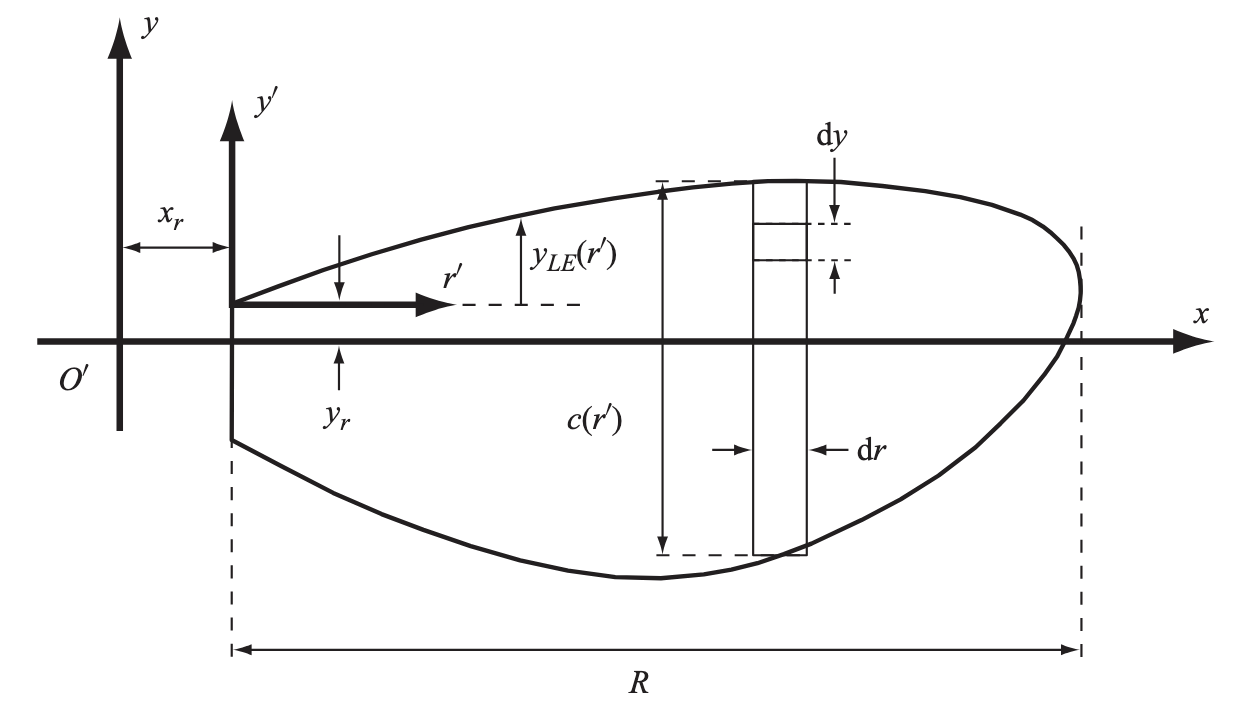
\includegraphics[width=0.60\textwidth]{planiform.png}
  \caption{Aeromechanical model of the RoboBee.}
  \label{fig:aeromechanical-model}
\end{wrapfigure}
Before starting, note the sign conventions, where \(+\phi\), \(+\omega_x\), and \(+\alpha\) are all positive for the local \(+x\) axis of the wing (i.e. pointing away from the root, along the hinge). For each strip, shown in Fig. \ref{fig:aeromechanical-model}, we have 
\begin{align}
    \label{eq:differential_lift_drag}
    \D F_{L} &= \frac{1}{2} \rho V_i^2 C_L(\alpha) c(r') \D r, \\
    \D F_{D} &= \frac{1}{2} \rho V_i^2 C_D(\alpha) c(r') \D r, 
\end{align}
where \(V_i = |\omega_h|(r + x_r)\). To derive this velocity, observe that a blade element has radial distance \(r + x_r\) (see Fig. \ref{fig:aeromechanical-model}). Then, the tangential speed (around the stroke, \(X'\) axis), is \(u(r) = |\omega_h| (r + x_r)\), so \(V_i^2 = \omega_h^2(r + x_r)^2\). Furthermore, \(c(r')\) is the chord length at the blade element, where \(r'\) is the distance from the wing root to the blade element. 
Then, the total lift is the integral over the wing span: 
\begin{align}
    F_L &= \int_0^R \D F_L \\ 
    &= \frac{1}{2} \rho \omega_h^2 C_L(\alpha)
    \underbrace{\int_0^R (r + x_r)^2 c(r') \D r}_{\hat{F}}, 
\end{align}
where \(\hat{F}\) is the dimensionless wing-shape factor. 
\begin{wrapfigure}{h!}{0.42\textwidth}
    \centering
    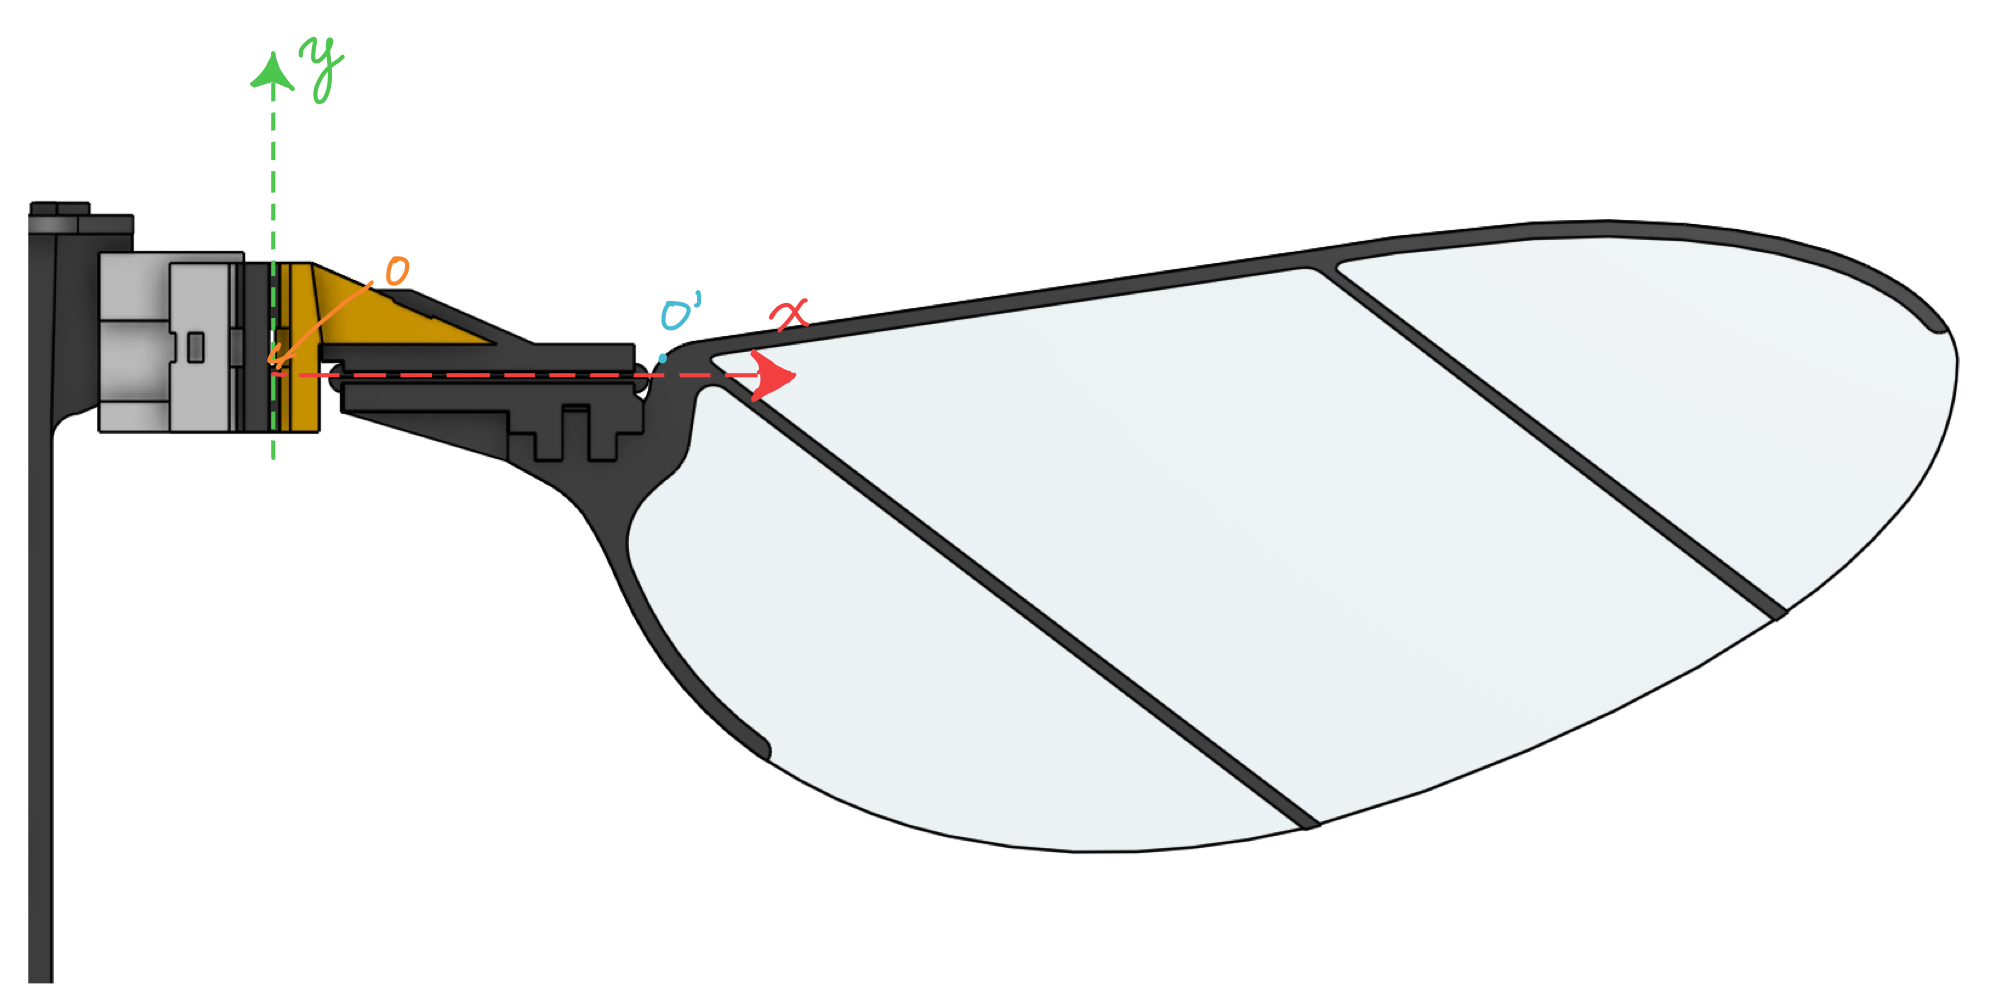
\includegraphics[width=\linewidth]{wing_coordinates.jpeg}
    \caption{Coordinate axes superimposed on CAD model.}
    \label{fig:coordinate_axes}
\end{wrapfigure}
Full derivation can be found in Appendix \ref{sec:non_dimensionalization_derivation}.
To non-dimensionalize the integral, set 
\begin{align}
    \hat{r} &= \frac{r'}{R}, \\
    \hat{x}_r &= \frac{x_r}{R}, \\
    \hat{c}(\hat{r}) &= \frac{c(r')}{\bar{c}},    
\end{align}
where \(\bar{c}\) is the mean chord length \(\frac{A}{R}\). (\(R\) is the wing span). 


\subsection{Compute aerodynamic pitch moment about the hinge}
\(M_{x,\mathrm{aero}}\) is combination of lift and drag forces, but as a moment. While the integral form given by Whitney and Wood is 
\begin{equation}
    M_{x,\mathrm{aero}} = \frac{1}{2} \rho \omega_h^2 C_N(\alpha) \int_0^R y_{cp}(r') (r' + x_r)^2 c(r') \D r'. 
\end{equation}
Note that \(\alpha\), the angle of attack. In discrete form, we have 
\begin{equation}
    M_{x,\mathrm{aero}} \approx \sum_{i=1}^{N} y_{cp,i} \D F_{N,i}. 
\end{equation}
Substituting in Eq. \ref{eq:differential_lift_drag}, then we have 
\begin{equation}
    M_{x,\mathrm{aero}} \approx -\sum_{i=1}^{N} \mathrm{sgn} (\alpha) y_{cp,i} \frac{1}{2} \rho V_i^2 C_N(\alpha_i) c_i \Delta r_i.
\end{equation}
Note the inclusion of \(\mathrm{sgn}\) because \(\textbf{F}_N = F_N \textbf{e}_N = -\mathrm{sgn}(\alpha) F_N \mathbf{e}_z\).
Here, \(y_{cp}(r')\) is the distance from the leading edge to the center of pressure for the blade element at \(r'\), and is given by 
\begin{equation}
    y_{cp} = y_r + y_{LE}(r') - c(r')\hat{d}_{cp}. 
\end{equation}
\(y_{LE}\) is basically the distance from the leading edge to the rotation axis, while \(\hat{d}_{cp}\) is the dimensionless distance (think: fraction) from the leading edge to the center of pressure, which is given by Dickson et al. (2006): 
\begin{equation}
    \hat{d}_{cp} = \frac{0.82}{\pi} |\alpha| + 0.05. 
\end{equation}

\subsection{Compute passive hinge restoring moment} 
\(M_{x, \mathrm{hinge}} = -\kappa_H \psi\) is a simple linear torsional spring model, where \(k\) is the torsional stiffness.
The torsial stiffness is given by 
\begin{equation}
    \kappa_H = \frac{E_h t_h^3 w_h}{12 L_h}, 
\end{equation}
where \(t_h = 0.0125\,\mathrm{mm}\), \(w_h = 2.7\,\mathrm{mm}\), and \(L_h = 0.10\,\mathrm{mm}\) are the thickness, width, and length of the central layer. For Kapton, \(E_h = 2.5\,\mathrm{GPa}\).
\subsection{Compute aerodynamic damping moment} 
\begin{equation}
    M_{x, \mathrm{rd}} = -\frac{1}{2} \rho \omega_x |\omega_x| C_{rd} \bar{c}^{4} R \hat{Y}_{rd}. 
\end{equation}
where
\begin{equation}
\hat{Y}_{rd}
=
\int_0^1 \hat{y}_{rd}(\hat{r})\,d\hat{r}.
\end{equation}
and 
\begin{equation}
\hat{y}_{rd}(\hat{r})
=
\frac{1}{4}
\left[
\left|\hat{y}_r + \hat{y}_{LE}\right|
\left(\hat{y}_r + \hat{y}_{LE}\right)^3
-
\left|\hat{y}_r + \hat{y}_{LE} - \hat{c}\right|
\left(\hat{y}_r + \hat{y}_{LE} - \hat{c}\right)^3
\right],
\end{equation}
the non-dimensional location of the effective moment arm of the rotational damping term. 
Set \(C_{\mathrm{rd}} = 2.0\) as the rotational damping moment coefficient. Again, \(\hat{y}_r\) is the dimensionless distance from the rotation axis to the root of the wing, while \(\hat{y}_{LE}\) is the dimensionless distance from the leading edge (outline of the wing planiform) to the rotation axis.

\subsection{Compute added mass effect moment}
The air inertia resisting wing acceleration, i.e. aerodynamic forces and moments that depend on the body's acceleration, adds another term to the total moment. Whitney and Wood start from the two-dimensional added-mass force and moment on a thin section. After dropping cross-terms that duplicate other quasi-steady blade-element terms, the reduced section equations are
\begin{align}
Z_0 &= -\lambda_z \dot{W}_0 - \lambda_{z\omega}\dot{\omega}_x, \\
Y_0 &= 0, \\
M_0 &= -\lambda_{z\omega}\dot{W}_0 - \lambda_{\omega}\dot{\omega}_x,
\end{align}
where \(Z_0\) is the added-mass normal force per unit span, \(M_0\) is the added-mass pitch moment per unit span, and
\begin{align}
\lambda_z &= \pi \rho a^2, \\
\lambda_{z\omega} &= -\pi \rho a^2 y_h, \\
\lambda_{\omega} &= \pi \rho a^2 y_h^2 + \frac{1}{8}\pi\rho a^4.
\end{align}
Here \(a=c(r')/2\) is the local semi-chord, and \(y_h\) is the signed offset from the torsional axis to the mid-chord of the local blade-element strip.

Using Whitney and Wood's kinematics, the local normal acceleration of the hinge line is
\begin{equation}
\dot{W}_0(r') = - (r' + x_r)\left(\dot{\omega}_y - \omega_x\omega_z\right),
\end{equation}
where \((r' + x_r)\) is the distance from the stroke-axis shoulder to the blade element. Radial integration of the reduced section moment gives
\begin{equation}
M_{x,am}
=
-
\left(
\frac{\pi}{4}\rho \bar{c}^{3} R^{2}\hat{I}_{xy,am}
\right)
\left(
\dot{\omega}_y - \omega_x\omega_z
\right)
-
\left(
\frac{\pi}{4}\rho \bar{c}^{4} R \hat{I}_{xx,am}
\right)
\dot{\omega}_x .
\end{equation}
Here, \(\hat{I}_{xy,\mathrm{am}}\) and \(\hat{I}_{xx,\mathrm{am}}\) are added-mass geometry integrals analogous to inertial products, and are constants found by
\begin{align}
\hat{I}_{xy,am}
&= \int_{0}^{1}
(\hat{r} + \hat{x}_r)\hat{c}(\hat{r})^2 \hat{y}_h(\hat{r}) \, d\hat{r}, \\[4pt]
\hat{I}_{xx,am}
&= \int_{0}^{1}
\hat{c}(\hat{r})^2
\left(
\hat{y}_h(\hat{r})^2 + \frac{1}{32}\hat{c}(\hat{r})^2
\right)
\, d\hat{r}.
\end{align}

\subsubsection{Applying added mass as a blade-element normal force}
\label{sec:added_mass_normal_force}
For a simulator that applies forces directly to the wing, the translational part of the added-mass effect can be applied strip-by-strip instead of only as a pre-integrated pitch moment. For blade element \(i\), with radial width \(\Delta r_i\), local chord \(c_i\), semi-chord \(a_i=c_i/2\), and signed mid-chord offset \(y_{h,i}\), compute
\begin{align}
\lambda_{z,i} &= \pi\rho a_i^2, \\
\lambda_{z\omega,i} &= -\pi\rho a_i^2 y_{h,i}, \\
\dot{W}_{0,i} &= -(r'_i+x_r)\left(\dot{\omega}_y-\omega_x\omega_z\right), \\
Z_{0,i} &= -\lambda_{z,i}\dot{W}_{0,i} - \lambda_{z\omega,i}\dot{\omega}_x .
\end{align}
The normal added-mass force on that strip is then
\begin{equation}
\Delta \mathbf{F}_{am,i} = Z_{0,i}\Delta r_i\,\mathbf{e}_z,
\label{eq:blade_added_mass_force}
\end{equation}
with the sign of \(Z_{0,i}\) carrying the direction along the local wing-fixed normal \(\mathbf{e}_z\). Depending on the simulator's force convention, this may need to be negated when converting from ``force of the air on the wing'' to ``reaction force of the wing on the body.''

The natural application point for this strip force is the local mid-chord location used by the added-mass section model,
\begin{equation}
\mathbf{p}_{am,i}
=
(r'_i+x_r)\mathbf{e}_x + y_{h,i}\mathbf{e}_y,
\label{eq:blade_added_mass_application_point}
\end{equation}
measured from the shoulder/hinge-frame origin. Applying Eq. \ref{eq:blade_added_mass_force} at Eq. \ref{eq:blade_added_mass_application_point} gives a pitch-axis moment contribution
\begin{equation}
\Delta M^{(F)}_{x,am,i}
=
 y_{h,i} Z_{0,i}\Delta r_i.
\end{equation}
This captures the moment induced by the translational added-mass normal force. To reproduce the full Whitney--Wood added-mass pitch moment, also include the local pure rotational added-mass couple
\begin{equation}
\Delta M^{(\omega)}_{x,am,i}
= -\lambda_{\omega,i}\dot{\omega}_x\Delta r_i,
\end{equation}
where
\begin{equation}
\lambda_{\omega,i}
=
\pi\rho a_i^2 y_{h,i}^2
+
\frac{1}{8}\pi\rho a_i^4.
\end{equation}
Thus, if using point forces only, Eq. \ref{eq:blade_added_mass_force} is the translational/normal added-mass load to apply to the strip. If matching the analytical rotational dynamics exactly, apply both the strip force and the additional strip torque/couple \(\Delta M^{(\omega)}_{x,am,i}\). Do not also add the pre-integrated \(M_{x,am}\) term as a scalar pitch moment when the strip force is active, or the force-induced moment will be double counted.

\subsection{Integration} 
\begin{equation}
    I_{xx}\ddot{\psi}
    = M_x
    + I_{xy}\ddot{\phi}\cos\psi
    + \frac{1}{2} I_{xx}\dot{\phi}^{2}\sin(2\psi).
\end{equation} 

\begin{equation}
    \ddot{\psi}
    =
    \frac{
        M_x
        + I_{xy}\ddot{\phi}\cos\psi
        + \frac{1}{2} I_{xx}\dot{\phi}^{2}\sin(2\psi)
    }{
        I_{xx}
    }, 
\end{equation}
where \(\ddot{\phi}\) is the stroke angular acceleration, which we can compute from the current stroke angle and velocity/actuator input. See Appendix \ref{sec:moment_of_inertia} for derivation of \(I_{xx}\) and \(I_{xy}\). In particular, assume \(\phi(t)\) (taken at transmission link 1) is commanded from the control algorithms (typically a sin wave with \(\omega = 170 \mathrm{Hz}\), i.e at resonance of transmission mechanism). This should be parametrized in the code. If added mass is applied as blade-element normal forces, the remaining scalar total moment is
\begin{equation}
    M_{\mathrm{total}}
    =
    M_{\mathrm{aero}}
    + M_{\mathrm{rot}}
    + M_{\mathrm{hinge}}
\end{equation}
But since aero forces originate as translational forces applied to the center of pressure, we can't just apply them purely as moments. 

So really, \(M_{\mathrm{aero}}\) needs to be applied as 
\begin{equation}
    \sum_i \mathbf{r}_{cp,i} \times \D \mathbf{F}_i, 
\end{equation}
where 
\begin{equation}
    \mathbf{r}_{cp,i} = (r+x_r)\mathbf{e}_x + y_{cp}(r)\mathbf{e}_y.
\end{equation}

\section{Lumped-Parameter Actuation Dynamics and Stroke Frequency Response}
\label{sec:lumped_actuation}

Everything above treats the stroke angle \(\phi(t)\) as given. In the current code it effectively is: the wing voltage maps algebraically to a slider displacement (\(2.5\,\mu\mathrm{m/V}\) about a \(100\,\mathrm{V}\) rest point) and a stiff PD joint actuator (\(K_p = 10^4\), \(K_d = 50\), effort limit \(10^9\,\mathrm{N}\)) forces the slider to track it. The stroke is therefore kinematically prescribed, and a frequency sweep of the present model would measure the tracking bandwidth of that servo rather than any physics. This section records how the transmission and actuator are modeled as a lumped second-order system in the literature, which of those lumped terms Drake already reproduces implicitly, and what has to be added so that the simulator can produce a stroke-amplitude frequency response \(|\Phi/V_{pp}|(\omega)\) of the kind shown in Steinmeyer et al., ``Yaw Torque Authority for a Flapping-Wing Micro-Aerial Vehicle'' (ICRA 2019), Fig.~3.

\subsection{Reference lumped model}
Following Finio et al. (2011) and Jafferis et al. (2016), Steinmeyer et al. model the actuator, transmission, and wing as one spring--mass--damper written on the actuator (slider) side. With actuator effective mass \(m_a\), actuator stiffness \(k_a\), transmission ratio \(T\) (rad of stroke per metre of slider travel), transmission flexure stiffness \(k_t\), wing moment of inertia about the stroke axis \(J_\phi\), and a linearized aerodynamic damping coefficient \(b\) acting at radius \(r_{cp}\),
\begin{align}
    m_{eq} &= m_a + T^2 J_\phi, \\
    b_{eq} &= T^2 r_{cp}\, b, \\
    k_{eq} &= k_a + T^2 k_t,
\end{align}
and the voltage-to-stroke transfer function is
\begin{equation}
    \label{eq:lumped_tf}
    H(\omega) = \frac{\Phi(\omega)}{V(\omega)} = \frac{A_H}{m_{eq}(\omega i)^2 + b_{eq}(\omega i) + k_{eq}},
\end{equation}
where \(A_H\) converts volts to slider force. Their Table~I values are \(m_a = 25\,\mathrm{mg}\), \(J_\phi = 51.1\,\mathrm{mg\,mm^2}\), \(T = 2666\), \(r_{cp} = 1.42\times 9.56\,\mathrm{mm}\), \(b = 2.03\times 10^{-6}\,\mu\mathrm{N\,s/m}\), \(k_a = 300\,\mathrm{N/m}\), \(k_t = 28.2\,\mu\mathrm{N\,m/rad}\), giving \(m_{eq} = 0.388\,\mathrm{g}\), \(b_{eq} = 0.196\,\mathrm{N\,s/m}\), \(k_{eq} = 500.4\,\mathrm{N/m}\) and a resonance near \(f_n = \frac{1}{2\pi}\sqrt{k_{eq}/m_{eq}} \approx 181\,\mathrm{Hz}\). Note that the wing term dominates: \(T^2 J_\phi \approx 363\,\mathrm{mg}\) versus \(m_a = 25\,\mathrm{mg}\), so about \(94\%\) of the equivalent mass is wing inertia reflected through the transmission. The resonant frequency is set almost entirely by \(J_\phi\) against \(T^2 k_t\).

This exact model is already implemented in MATLAB as \texttt{simulink/system id/get\_transfer\_function.m} with the Table~I parameters in \texttt{data\_optimize\_full\_optimization.m}, but it is only ever evaluated at two discrete frequencies and is not connected to the Drake plant. Plotting Eq.~\eqref{eq:lumped_tf} over \(50\)--\(400\,\mathrm{Hz}\) from that function is the analytic reference curve that the simulator result below should be compared against.

\subsection{Mapping of lumped terms onto the Drake plant}
The point of doing this in Drake rather than with Eq.~\eqref{eq:lumped_tf} is that several of the lumped parameters stop being parameters and become consequences of the geometry and the aerodynamics already in the model. Table~\ref{tab:lumped_map} summarizes the mapping.

\begin{table}[H]
\centering
\begin{tabular}{l l l}
\hline
Lumped term & Drake representation & Status \\
\hline
\(T\) (transmission ratio) & Emergent from four-bar linkage kinematics & Done \\
\(J_\phi\) (wing inertia) & Rigid-body inertia of hinge/frame/membrane bodies & Done \\
\(b\) (aero damping) & Blade-element drag reacting through linkage & Done \\
\(m_a\) (actuator mass) & Reflected inertia on slider actuator & To do \\
\(k_a\) (actuator stiffness) & \texttt{PrismaticSpring} on slider joint & To do \\
\(A_H V\) (voltage force) & Pure force on slider actuation input & To do \\
\(k_t\) (flexure stiffness) & \texttt{RevoluteSpring} on stroke joint(s) & To do \\
\hline
\end{tabular}
\caption{Correspondence between the Steinmeyer et al. lumped parameters and the Drake plant.}
\label{tab:lumped_map}
\end{table}

\subsubsection{Transmission ratio (done)}
The transmission is a real closed-loop mechanism in the \texttt{MultibodyPlant}: \texttt{slider\_2} (prismatic, the actuator tip surrogate) drives \texttt{transmission\_link\_1}, which connects through \texttt{transmission\_link\_2} and the loop-closure ball constraints to \texttt{transmission\_hinge}, whose joint \texttt{revolute\_1\_3} is the stroke angle \(\phi\) for the left wing (\texttt{slider\_1} / \texttt{revolute\_1\_4} for the right). \(T\) is therefore the local slope \(\partial\phi/\partial x_{slider}\) of the forward kinematics, including its nonlinearity at large stroke, and does not need to be specified.

\subsubsection{Wing inertia (done)}
\(J_\phi\) enters the lumped model only through \(m_{eq}\). In Drake the same quantity arises because the transmission hinge, hinge base, hinge wing, carbon-fibre frame, and membrane are rigid bodies carried by the stroke joint. Walking the URDF chain from \texttt{transmission\_hinge} at zero joint angle and applying the parallel-axis theorem about the stroke axis gives, per wing,
\begin{table}[H]
\centering
\begin{tabular}{l r r r}
\hline
Body & mass (mg) & \(r_\perp\) from stroke axis (mm) & \(J\) (mg\,mm\(^2\)) \\
\hline
\texttt{wing\_cf} & 0.614 & 7.42 & 43.2 \\
\texttt{wing\_membrane} & 0.077 & 9.23 & 7.4 \\
\texttt{hinge\_left\_wing} & 0.514 & 2.36 & 3.2 \\
\texttt{hinge\_left\_base} & 0.418 & 1.76 & 1.6 \\
\texttt{transmission\_hinge} + \texttt{link\_2} & 1.256 & \(\sim\)0.6 & 0.7 \\
\hline
Total & 2.879 & & 56.0 \\
\hline
\end{tabular}
\caption{URDF wing inertia about the stroke axis, left wing; the right wing is identical to three figures. Compare \(J_\phi = 51.1\,\mathrm{mg\,mm^2}\) in Steinmeyer et al.}
\label{tab:stroke_inertia}
\end{table}
The URDF value is \(10\%\) above the paper's, which by itself would move the predicted resonance from \(181\) to about \(173\,\mathrm{Hz}\). This is within the robot-to-robot spread reported in that paper. Because \(J_\phi\) is \(94\%\) of \(m_{eq}\), this table is the single most important input to the resonant frequency and should be re-checked whenever the wing URDF changes. Note also that the added-mass normal force of Section~\ref{sec:added_mass_normal_force} acts as an additional effective inertia that the lumped model does not separate out; the simulated \(m_{eq}\) will read slightly higher than the rigid-body number.

\subsubsection{Aerodynamic damping (done, but quadratic)}
The blade-element wrench is applied as a full six-component spatial force on the wing body, so its stroke-axis moment reacts back through the linkage to the slider and is exactly the load the actuator must overcome. This is the physical origin of \(b\). Two caveats. First, the only explicitly authored rotational damping term \(M_{x,\mathrm{rd}}\) acts about the span (pitch) axis, not the stroke axis; stroke damping comes purely from the drag moments \(\sum_i \mathbf{r}_{cp,i}\times\D\mathbf{F}_i\). Second, drag scales with \(\dot{\phi}|\dot{\phi}|\) whereas the lumped \(b\) is a linearization. The simulated frequency response is therefore amplitude-dependent: the resonance peak will be taller and narrower at small \(V_{pp}\) and flatter at flight voltage. The comparison with Eq.~\eqref{eq:lumped_tf} holds at one amplitude only, and the sweep should be run at several.

\subsubsection{Actuator mass (to do)}
The piezo bimorph layers in the URDF are welded to the airframe and never move; the slider link that stands in for the actuator tip weighs \(0.3\,\mathrm{mg}\), not the \(25\,\mathrm{mg}\) effective modal mass of the cantilever. The cleanest fix is Drake's actuator reflected inertia: \texttt{JointActuator::set\_default\_rotor\_inertia} and \texttt{set\_default\_gear\_ratio} add \(I_{rotor}\,n^2\) to the joint degree of freedom, which for a prismatic joint has units of mass. Setting \(I_{rotor} = 25\times 10^{-6}\,\mathrm{kg}\) and \(n = 1\) on each slider actuator adds exactly \(m_a\) without altering gravity loads, centre of mass, or the loop-closure geometry. The alternative of raising the \texttt{transmission\_link\_1} mass in the URDF also works but shifts the body COM. Since \(m_a\) is only \(6\%\) of \(m_{eq}\), omitting it costs about \(3\%\) in \(f_n\); it is included for completeness rather than because it moves the answer.

\subsubsection{Actuator stiffness and voltage force (to do)}
The standard lumped description of a piezo bending actuator is a spring to ground whose equilibrium shifts with voltage,
\begin{equation}
    F_{tip} = k_a\bigl(\delta_{free}(V) - x\bigr), \qquad \delta_{free}(V) = c_V\,(V - V_{rest}),
\end{equation}
with \(c_V = 2.5\times 10^{-6}\,\mathrm{m/V}\) and \(V_{rest} = 100\,\mathrm{V}\) as currently coded. This is not a series arrangement; it decomposes into two elements acting in parallel on the same slider degree of freedom:
\begin{itemize}
    \item a \texttt{PrismaticSpring} force element on each slider joint with stiffness \(k_a = 300\,\mathrm{N/m}\) and nominal position equal to the slider rest position read from the default context after \texttt{Finalize};
    \item a pure force input \(u = k_a c_V (V - V_{rest})\) fed to the plant's actuation input port.
\end{itemize}
Concretely, the existing slider \texttt{JointActuator}s are kept but \texttt{set\_controller\_gains} is no longer called, so they become pure force actuators, and the effort limit is set to the blocking force \(k_a\,c_V\,\Delta V_{max} \approx 300 \times 0.25\times 10^{-3} \approx 75\,\mathrm{mN}\) instead of \(10^9\,\mathrm{N}\). \texttt{VoltageStrokeSource} changes from emitting a four-vector desired state \([q_1, q_2, v_1, v_2]\) to emitting a two-vector of forces, and is connected to \texttt{get\_actuation\_input\_port()} instead of the desired-state port. The voltage-derivative inputs it currently consumes become unnecessary. The commented-out \(0.1\,\mathrm{N}\) effort limit already present in the source suggests this direction was anticipated.

\subsubsection{Transmission flexure stiffness (to do)}
The lumped \(k_t\) is one torsional stiffness at the output angle; physically the four-bar has a flexure at every joint. Two passes are planned:
\begin{enumerate}
    \item \textbf{Matching the paper.} One \texttt{RevoluteSpring} on each stroke output joint, \texttt{revolute\_1\_3} and \texttt{revolute\_1\_4}, with \(k_t = 28.2\,\mu\mathrm{N\,m/rad}\), following the pattern of \texttt{AddWingHingeSprings}. The nominal angle must be the stroke angle at slider rest, read from the default context, not assumed zero. This is the apples-to-apples comparison with Eq.~\eqref{eq:lumped_tf}.
    \item \textbf{Distributed flexures.} Assign each revolute joint in the linkage chain its own stiffness from the same Kapton flexure formula used for the wing hinge, \(\kappa = E t^3 w / 12L\), with that flexure's geometry. The loop-closure joints are modeled as ball constraints rather than joints and cannot carry springs, so the stiffness must be placed on the revolute joints only. With this pass \(k_t\) becomes emergent in the same way \(T\) already is.
\end{enumerate}
No damping is authored on the transmission or slider. The real actuator has some material damping; a small slider joint damping may also be needed for numerical reasons once the PD gains that currently stiffen the loop-closure constraints are removed (see Section~\ref{sec:lumped_validation}).

\subsection{Sweep infrastructure (to do)}
Three things are required before any frequency response can be plotted:
\begin{itemize}
    \item \(f_{drive}\) is a compile-time constant (\texttt{kDriveFrequencyHz = 180}) in two places in \texttt{visualize\_robobee\_aeromechanical.cc}, and the plant time step is derived from it as \(1/(100 f_{drive})\). Promote the frequency to a runtime flag and fix the time step independently, at roughly \(2\times 10^{-5}\,\mathrm{s}\) so the highest swept frequency (\(400\,\mathrm{Hz}\)) still has \(\sim 50\) steps per cycle.
    \item Nothing logs \(\phi\). Add the stroke angles from \texttt{revolute\_1\_3} and \texttt{revolute\_1\_4} to the slider CSV alongside slider position and voltage. The Simulink TCP response packet also carries no wing joint state, so the sweep should be driven from the standalone app, not over TCP.
    \item A driver script that runs the sweep over \(50\)--\(400\,\mathrm{Hz}\) in \(5\)--\(10\,\mathrm{Hz}\) steps at fixed \(V_{pp}\), discards \(\sim 20\) cycles of transient, fits the amplitude at the drive frequency, and plots \(|\Phi/V_{pp}|\) against frequency with the analytic curve from \texttt{get\_transfer\_function.m} overlaid. Repeat at two or three values of \(V_{pp}\) to expose the amplitude dependence of the quadratic damping.
\end{itemize}

\subsection{Validation before sweeping}
\label{sec:lumped_validation}
Apply a static voltage step and record the steady-state slider displacement \(x_{ss}\) and stroke angle \(\phi_{ss}\). Two checks follow:
\begin{align}
    \frac{x_{ss}}{\delta_{free}} &= \frac{k_a}{k_a + T^2 k_t} = \frac{k_a}{k_{eq}} \approx 0.60, \\
    \frac{\phi_{ss}}{x_{ss}} &= T \approx 2666\,\mathrm{rad/m}.
\end{align}
If either is far off, the spring nominal positions or the loop-closure constraint compliance are wrong and a frequency sweep would be meaningless. This test also reveals whether the SAP solver remains well behaved through the loop-closure constraints once the stiff PD gains are removed; constraint chatter at this stage is the signal to add slider damping.

Once the sweep matches the analytic reference at small amplitude, the simulated \(H(\omega)\) can be used to reproduce the split-cycle filtering result (Steinmeyer et al.\ Fig.~4) directly, by driving the second-harmonic waveform \(V(t) = V_{amp}[a_1\sin\omega t \pm a_2\sin 2\omega t + a_3 \sin 3\omega t]\) and comparing the resulting \(\phi(t)\) upstroke and downstroke speeds.

\subsection{Order of work}
\begin{enumerate}
    \item Analytic reference curve from \texttt{get\_transfer\_function.m} over \(50\)--\(400\,\mathrm{Hz}\).
    \item Plant changes in the standalone app: reflected inertia, \texttt{PrismaticSpring}, single \texttt{RevoluteSpring} per stroke joint, pure-force slider actuation.
    \item Static validation of \(T\) and \(k_a/k_{eq}\).
    \item Frequency flag, \(\phi\) logging, sweep driver, Bode plot against the reference.
    \item Amplitude dependence, then distributed flexure stiffness, then the split-cycle waveform test.
\end{enumerate}
The TCP server path used by Simulink stays on the position servo until the standalone version validates.

\section{Conclusion and Open Questions}


\section{Appendix} 
\subsection{Change of Basis Derivation} 
\label{sec:change_of_basis_derivation}
The derivation is a change of basis from the mixed-frame angular velocity
\begin{equation}
    \boldsymbol{\omega}
    = -\dot{\phi}\,\mathbf{e}_{X'}
      + \dot{\theta}\,\mathbf{e}_{z'}
      + \dot{\psi}\,\mathbf{e}_x
\end{equation}
to the wing-fixed basis \((\mathbf{e}_x, \mathbf{e}_y, \mathbf{e}_z)\).
Using the paper's sign convention,
\begin{align}
    \mathbf{e}_{z'}
        &= \sin\psi\,\mathbf{e}_y + \cos\psi\,\mathbf{e}_z, \\
    \mathbf{e}_{X'}
        &= \sin\theta\,\mathbf{e}_x
           + \cos\theta
             \left(\cos\psi\,\mathbf{e}_y
             - \sin\psi\,\mathbf{e}_z\right).
\end{align}
Substitution gives
\begin{align}
    \boldsymbol{\omega}
        &= -\dot{\phi}
           \left[
             \sin\theta\,\mathbf{e}_x
             + \cos\theta
               \left(\cos\psi\,\mathbf{e}_y
               - \sin\psi\,\mathbf{e}_z\right)
           \right] \nonumber \\
        &\quad
           + \dot{\theta}
             \left(\sin\psi\,\mathbf{e}_y
             + \cos\psi\,\mathbf{e}_z\right)
           + \dot{\psi}\,\mathbf{e}_x \nonumber \\
        &= \left(\dot{\psi} - \dot{\phi}\sin\theta\right)\mathbf{e}_x
           + \left(-\dot{\phi}\cos\theta\cos\psi
             + \dot{\theta}\sin\psi\right)\mathbf{e}_y \nonumber \\
        &\quad
           + \left(\dot{\phi}\cos\theta\sin\psi
             + \dot{\theta}\cos\psi\right)\mathbf{e}_z .
\end{align}
Therefore, the wing-fixed angular velocity components are
\begin{align}
    \omega_x &= \dot{\psi} - \dot{\phi}\sin\theta, \\
    \omega_y &= -\dot{\phi}\cos\theta\cos\psi
                + \dot{\theta}\sin\psi, \\
    \omega_z &= \dot{\phi}\cos\theta\sin\psi
                + \dot{\theta}\cos\psi .
\end{align}
The \(-\dot{\phi}\sin\theta\) term in \(\omega_x\) appears because wing deviation projects part of the flapping angular velocity onto the wing pitch axis. In the planar case, \(\theta = 0\), so \(\omega_x = \dot{\psi}\).

\subsection{Non-dimensionalization Derivation} 
\label{sec:non_dimensionalization_derivation} 
Start with the dimensional spanwise integral from the lift expression:
\begin{equation}
    I_F = \int_0^R (r + x_r)^2 c(r') \D r.
\end{equation}
Here \(r\) is the spanwise coordinate used in the blade-element integral, and
\(r'\) is the same physical distance measured from the wing root for evaluating
the local chord distribution. Thus, for this simplified planar wing model, we
take \(r' = r\).

Using the normalized dimensions for the distance along the wing root, the distance from the wing root to the rotation axis, and the chord length, 
\begin{align}
    \hat{r} &= \frac{r}{R}, &
    \hat{x}_r &= \frac{x_r}{R}, &
    \hat{c}(\hat{r}) &= \frac{c(r)}{\bar{c}},
\end{align}
we have
\begin{align}
    r &= R\hat{r}, &
    x_r &= R\hat{x}_r, &
    c(r) &= \bar{c}\hat{c}(\hat{r}), &
    \D r &= R \D \hat{r}.
\end{align}
Note that \((x_r, y_r)\) are the coordinates of the root of the wing (which is basically the hinge). Substituting these into \(I_F\) gives
\begin{align}
    I_F
        &= \int_0^1
           \left(R\hat{r} + R\hat{x}_r\right)^2
           \bar{c}\hat{c}(\hat{r})
           R \D \hat{r} \\
        &= R^3\bar{c}
           \int_0^1
           \left(\hat{r} + \hat{x}_r\right)^2
           \hat{c}(\hat{r}) \D \hat{r}.
\end{align}
Therefore, the nondimensionalized integral is
\begin{equation}
    \hat{F}
        = \frac{I_F}{R^3\bar{c}}
        = \int_0^1
          \left(\hat{r} + \hat{x}_r\right)^2
          \hat{c}(\hat{r}) \D \hat{r}.
\end{equation}
Expanding the square,
\begin{align}
    \hat{F}
        &= \int_0^1
           \left(\hat{r}^2
           + 2\hat{x}_r\hat{r}
           + \hat{x}_r^2\right)
           \hat{c}(\hat{r}) \D \hat{r} \\
        &= \int_0^1 \hat{r}^2\hat{c}(\hat{r}) \D \hat{r}
           + 2\hat{x}_r
             \int_0^1 \hat{r}\hat{c}(\hat{r}) \D \hat{r}
           + \hat{x}_r^2
             \int_0^1 \hat{c}(\hat{r}) \D \hat{r}.
\end{align}
Since \(\bar{c} = A/R\),
\begin{equation}
    \int_0^1 \hat{c}(\hat{r}) \D \hat{r}
        = \frac{1}{R\bar{c}}\int_0^R c(r) \D r
        = \frac{A}{R\bar{c}}
        = 1.
\end{equation}
Define the nondimensional radius moments by
\begin{align}
    \hat{r}_1
        &= \int_0^1 \hat{r}\hat{c}(\hat{r}) \D \hat{r}, \\
    \hat{r}_2^2
        &= \int_0^1 \hat{r}^2\hat{c}(\hat{r}) \D \hat{r}.
\end{align}
Then the compact form is
\begin{equation}
    \hat{F}
        = \hat{r}_2^2
          + 2\hat{x}_r\hat{r}_1
          + \hat{x}_r^2.
\end{equation}

\section{Moment of Inertia Derivation}
\label{sec:moment_of_inertia} 
The moment of inertia for the left wing \(I_{xx,\mathrm{CM}} = 1.3 \times 10^{-6}\) and \(I_{xy,\mathrm{CM}} = 2.25 \times 10^{-7}\), from the CAD model, and around the center of mass. All other elements of the matrix can be approximated as 0 for this pitch equation. However, these need to be expressed around the pitch hinge axis. Assuming the CAD axes are already aligned with the wing-fixed axes used in the derivation, the tensor parallel axis theorem tells us that 
\begin{equation}
I_H
=
I_{CM}
+
m\left((\mathbf{d}^T \mathbf{d})\mathbf{1} - \mathbf{d}\mathbf{d}^T\right),
\end{equation}
where \(m\) is the wing mass, \(\mathbf{1}\) is the \(3 \times 3\) identity matrix, and \(\mathbf{d}\) is the displacement vector from the wing center of mass to the pitch hinge origin, expressed in the same wing-fixed frame as \(I_{CM}\). The displacement vector is
\begin{equation}
\mathbf{d}
=
\begin{bmatrix}
d_x \\
d_y \\
d_z
\end{bmatrix}
=
\begin{bmatrix}
-7.6171 \\
-0.5949 \\
0.000
\end{bmatrix}.
\end{equation}
All distances must be in units consistent with the CAD inertia units. If the inertia is used in SI units, then the displacement vector should be converted from millimeters to meters before applying the theorem.

Expanding the parallel-axis term gives
\begin{equation}
(\mathbf{d}^T \mathbf{d})\mathbf{1} - \mathbf{d}\mathbf{d}^T
=
\begin{bmatrix}
d_y^2 + d_z^2 & -d_xd_y & -d_xd_z \\
-d_yd_x & d_x^2 + d_z^2 & -d_yd_z \\
-d_zd_x & -d_zd_y & d_x^2 + d_y^2
\end{bmatrix}.
\end{equation}
Therefore, the hinge-frame inertia components needed by the pitch equation are
\begin{align}
I_{xx,H}
&=
I_{xx,\mathrm{CM}} + m(d_y^2 + d_z^2), \\
I_{xy,H}
&=
I_{xy,\mathrm{CM}} - m d_x d_y.
\end{align}
Substituting the displacement vector above,
\begin{align}
I_{xx,H}
&=
1.3 \times 10^{-6}
+ m\left((-0.5949)^2 + 0^2\right), \\
I_{xy,H}
&=
2.25 \times 10^{-7}
- m(-7.6171)(-0.5949).
\end{align}
Equivalently, using the millimeter CAD coordinates as written,
\begin{align}
I_{xx,H}
&=
1.3 \times 10^{-6}
+ 0.35390601\,m, \\
I_{xy,H}
&=
2.25 \times 10^{-7}
- 4.53141279\,m.
\end{align}
These are the constants to use for \(I_{xx}\) and \(I_{xy}\) in the pitch dynamics equation:
\begin{align}
I_{xx} &= I_{xx,H}, \\
I_{xy} &= I_{xy,H}.
\end{align}
If the CAD inertia tensor is reported in a frame that is rotated relative to the wing-fixed frame, first rotate it into the wing-fixed frame,
\begin{equation}
I_{CM}^{wing}
=
R I_{CM}^{CAD} R^T,
\end{equation}
and then apply the parallel axis theorem above.
\end{document}
